\documentclass[conference]{IEEEtran}
\IEEEoverridecommandlockouts
\usepackage{cite}
\usepackage{amsmath,amssymb,amsfonts}
\usepackage{algorithmic}
\usepackage{graphicx}
\usepackage{textcomp}
\usepackage{xcolor}
\usepackage{array}
\usepackage{multirow}
\usepackage{url}
\usepackage{tikz}
\usetikzlibrary{positioning,arrows.meta,shapes.geometric,calc}
\def\BibTeX{{\rm B\kern-.05em{\sc i\kern-.025em b}\kern-.08em
    T\kern-.1667em\lower.7ex\hbox{E}\kern-.125emX}}

\begin{document}

\title{A Single-Asset, Edge-First Digital Twin for Non-Invasive
Condition Monitoring of Legacy MSME Machinery}

\author{
\IEEEauthorblockN{1\textsuperscript{st} Samarth D Kolur}
\IEEEauthorblockA{\textit{Dept. of Computer Science}\\
\textit{and Technology}\\
\textit{Dayananda Sagar University}\\
Bengaluru, India\\
samarthdkolur1@gmail.com}
\and
\IEEEauthorblockN{2\textsuperscript{nd} Manoj C}
\IEEEauthorblockA{\textit{Dept. of Computer Science}\\
\textit{and Technology}\\
\textit{Dayananda Sagar University}\\
Bengaluru, India\\
manojchandrashekhar.058@gmail.com}
\and
\IEEEauthorblockN{3\textsuperscript{rd} Yashaswini R}
\IEEEauthorblockA{\textit{Dept. of Computer Science}\\
\textit{and Technology}\\
\textit{Dayananda Sagar University}\\
Bengaluru, India\\
rygowda1703@gmail.com}
\and
\IEEEauthorblockN{4\textsuperscript{th} Dr. Ramandeep Kaur}
\IEEEauthorblockA{\textit{Dept. of Computer Science}\\
\textit{and Technology}\\
\textit{Dayananda Sagar University}\\
Bengaluru, India\\
ramandeep-ct@dsu.edu.in}
\and
\IEEEauthorblockN{5\textsuperscript{th} Dr. Danthuluri Sudha}
\IEEEauthorblockA{\textit{Dept. of Computer Science}\\
\textit{and Technology}\\
\textit{Dayananda Sagar University}\\
Bengaluru, India\\
danthulurisudha15@gmail.com}
}

\maketitle

\begin{abstract}
Micro, Small and Medium Enterprises (MSMEs) contribute 30.1\% of India's
gross domestic product and 45.73\% of its exports, yet most of their
production assets are legacy machines with no industrial data interface of
the kind commercial digital twin platforms presuppose. This paper presents
Digital Cousin, a twin built on three properties: single-asset in scope,
edge-first in execution, natural-language accessible in interface. This
paper reports Phase~1, its monitoring foundation.
One rotary machine is retrofitted non-invasively with a MEMS accelerometer
and a 1-Wire temperature probe. A 64-sample burst at a configured 800~Hz
output data rate is reduced on-device to four AC-coupled statistical
features, and a single five-second publish cycle persists both sensor
channels at a measured 0.2~Hz into two separate SQLite tables. The resulting state
object has exactly one writer and leaves its model-derived fields explicitly
null, so Phase~2 populates them without a schema migration. A local REST
service and an offline-capable dashboard render live telemetry and
deterministic threshold alerts with no network egress. Deployment costs
approximately INR 20,000 in one-time hardware, with no licence and no cloud
dependency. We report the architecture, the retrofit protocol, the
evaluation plan and the bring-up findings that amended it.
\end{abstract}

\begin{IEEEkeywords}
digital twin, digital shadow, MSME, brownfield retrofit, edge computing,
Internet of Things, MQTT, offline-first systems, vibration monitoring,
Industry 4.0
\end{IEEEkeywords}

\section{Introduction}

India's MSME sector is the structural base of the country's manufacturing
output, contributing 30.1\% of national GDP and 45.73\% of exports
\cite{b36}. It is also the least instrumented part of that economy: its
capital stock is dominated by lathes, compressors, pumps and induction
motors that predate any industrial data interface, and the headroom to
replace them does not exist, with MSME credit demand at roughly INR 69.3
lakh crore against a formal supply near INR 14.5 lakh crore \cite{b37}.

Digital twin technology has matured over the same period \cite{b1}, with
reference architectures for twin-based predictive maintenance \cite{b3}
built on the five-level cyber-physical hierarchy \cite{b2}. These are sound
and also inapplicable here, because each assumes structured telemetry over
OPC-UA, MTConnect, Modbus or a vendor-native stack, and a legacy lathe emits
none of these \cite{b4}. The barrier is not the price of the twin but the
absence of anything for the twin to read.

Five structural barriers govern the setting, and the architecture of
Section~\ref{sec:arch} responds to each: the \emph{cost} of a commercial
suite's outlay and recurring licence; the \emph{brownfield} absence of a
protocol interface; the \emph{skill} barrier, since a dashboard of kurtosis
trends presumes a reader a ten-person workshop generally lacks; the
\emph{scale mismatch} of a whole-factory twin deployed against a firm
depending on one asset; and the \emph{connectivity} assumption of a reliable
uplink such a workshop lacks. Adoption studies locate the binding constraint
in the absence of an affordable implementation path \cite{b33} rather than
in awareness \cite{b34}.

The programme runs in two phases. Phase~1, reported here, establishes the
retrofit, the edge acquisition path and the digital shadow that make the
asset legible at all; Phase~2, scoped in Section~\ref{sec:conc}, adds
on-device analytics and the language interface. The contributions of
Phase~1 are: a formal three-property paradigm, argued in
Section~\ref{sec:para} to be a distinct design point rather than a degraded
enterprise twin; a four-layer architecture and retrofit protocol with a
published bill of materials of approximately INR 20,000 and no recurring
cost (Section~\ref{sec:arch}); a deterministic pipeline reducing a
64-sample burst at a configured 800~Hz to four AC-coupled features; and a
canonical state object as an immutable contract with one writer and model
fields explicitly null, so no consumer can mistake an absent model output
for a measurement (Section~\ref{sec:state}).

\section{Related Work}

\subsection{Digital Twin Architectures for Constrained Settings}

The literature is organised around physical--cyber integration \cite{b1}
and the 5C hierarchy \cite{b2}. Van Dinter et al.\ synthesised 42
twin-based predictive maintenance studies into a reference architecture
\cite{b3} whose applicability begins where structured telemetry already
exists, and Leng et al.\ showed twin cost is compressible via
open-architecture tools and REST middleware \cite{b4}, though on tools
designed to be read. Closest to this setting is Krommes and Tomaschko's
framework for brownfield SME production \cite{b5}; it reaches monitoring but
not predictive analytics or an operator-facing interface. Gautam et al.\
standardise legacy data through MTConnect under a four-agent LLM interface
\cite{b6}, but require an MTConnect-capable server and a cloud-hosted
model.

\subsection{Bearing Diagnostics and the Choice of Features}

Rolling-element bearing diagnosis is the best-characterised failure mode in
rotary machinery and sets the requirement the acquisition path must meet.
Its signal-processing basis, including spectral kurtosis band selection and
envelope analysis \cite{b9}, also establishes what a low-rate path cannot
see: RMS, kurtosis, crest factor and peak-to-peak are computable from a
short burst and stay informative for low- and mid-frequency degradation,
whereas envelope analysis of high-frequency signatures does not survive the
rate reduction. Two datasets dominate and are named here as Phase~2 training
sources: CWRU, whose benchmark study establishes that records differ in
diagnosability and some are not reliably diagnosable at all \cite{b7}, and
the IMS run-to-failure set \cite{b8}. Deep architectures on them report very
high accuracy \cite{b10,b11,b13}, but at 12~kHz and above on server-class
compute, which a sub-INR-300 MEMS accelerometer on a Pi cannot supply. The
Isolation Forest \cite{b12}, cheap enough for a microcontroller and needing
no fault history, is the baseline Phase~2 adopts.

\subsection{Edge Inference and TinyML}

Reviews of the TinyML stack for predictive maintenance find attention
unevenly distributed, models well served while data optimisation and
representative datasets are not \cite{b15}, and conclude it is a plausible
bridge for resource-constrained settings but lacks a demonstrated end-to-end
MSME deployment \cite{b35}. Three systems bound the achievable envelope: an
unsupervised Isolation Forest on an ESP32 inferring under 16~ms in 80~KB of
RAM without labelled faults \cite{b16}; LOPdM, needing neither mains power
nor a network \cite{b17}; and LiRUL, fitting prognostics into an edge budget
at 0.15M parameters \cite{b20}. None provides an operator interface: each
ends at an anomaly flag or a scalar, assuming a trained technician will read
it. Industrial LLM work supplies one but moves the computation off the
device \cite{b24,b25,b26}, and Xia et al.\ caution that current models lack
the deterministic fidelity autonomous intervention would require \cite{b27}.
We scope the Phase~2 interface to be read-only accordingly.

\subsection{Positioning}

Table~\ref{tab:gap} scores representative prior work against the five
properties this deployment requires. Several works satisfy three; we are not
aware of any satisfying all five, and that unoccupied intersection is what
the programme targets. Phase~1 demonstrates four, and P4 is the Phase~2
deliverable.

\begin{table}[t]
\caption{Representative Prior Work Against the Five Required Properties}
\label{tab:gap}
\centering
\footnotesize
\setlength{\tabcolsep}{4pt}
\begin{tabular}{|l|c|c|c|c|c|}
\hline
\textbf{Work} & \textbf{P1} & \textbf{P2} & \textbf{P3} & \textbf{P4} & \textbf{P5} \\
\hline
Reference twin architectures \cite{b1,b2,b3} & N & N & N & N & N \\
Low-cost twin reconfiguration \cite{b4} & N & N & N & N & P \\
Brownfield SME twin \cite{b5}     & N & N & P & N & P \\
Legacy twin with LLM \cite{b6}    & N & N & P & Y & N \\
Server-class diagnosis \cite{b10,b11,b13} & Y & P & N & N & N \\
TinyML PdM reviews \cite{b15,b35} & P & Y & P & N & Y \\
Edge monitors \cite{b16,b17,b20}  & Y & Y & N & N & Y \\
Edge SLM frameworks \cite{b23}    & N & Y & N & P & Y \\
Cloud industrial LLM \cite{b24,b25,b26,b27} & Y & N & N & Y & N \\
\hline
\textbf{Digital Cousin (Phase 1)} & \textbf{Y} & \textbf{Y} & \textbf{Y} & \textbf{P} & \textbf{Y} \\
\hline
\multicolumn{6}{p{0.95\columnwidth}}{\scriptsize Y demonstrated, P partially
addressed or carrying a structural dependency that limits transfer, N not
addressed. \textbf{P1} single-asset scope; \textbf{P2} edge-only execution;
\textbf{P3} MSME context; \textbf{P4} natural-language interface;
\textbf{P5} low-cost hardware. Our P4 is P because Phase~1 delivers the
state contract the interface consumes; the interface is Phase~2.} \\
\end{tabular}
\end{table}

\section{The Digital Cousin Paradigm}
\label{sec:para}

We use \emph{cousin} rather than \emph{twin} deliberately. A twin connotes
fidelity: a replica close enough to stand in for its counterpart in
simulation. Nothing here attempts that. What it offers is a partial,
deliberately narrow relative of the asset, with enough shared structure to
answer one question usefully and no pretence of completeness.

\textbf{P1, single-asset scope.} The unit of deployment is exactly one
machine, the bottleneck or highest-consequence failure point. That is a
positive design choice, not budget-driven truncation. Plant-wide
architectures spend their complexity on topology, asset registries and
multi-tenant data models, all overhead for a firm whose production depends
on one lathe. Narrowing to one asset collapses the state model to a single
object and brings the compute budget inside a single-board computer.

\textbf{P2, edge-first execution.} Acquisition, feature extraction, storage,
alerting and the dashboard all execute on the edge node with no network
egress. Cloud connectivity is an optional accelerator for the Phase~2
interface, never a dependency. This distinguishes the design from edge-assisted
architectures that localise inference but retain the cloud for retraining or
visualisation, which an intermittent industrial connection degrades to
unavailability.

\textbf{P3, natural-language accessibility.} The operator's primary
interface is intended to be a question in their own words, answered in plain
language; the dashboard is retained for the owner and technician. This is
the Phase~2 deliverable, and stating it here is not decoration, because it
imposes two obligations on Phase~1: machine state must be retrievable as
structured data rather than reconstructed from a rendering, and an interface
that cannot be cross-checked against a chart must never state a number it
did not retrieve. Both are why the state object is the system's contract
rather than an artefact of the dashboard, and why it separates a null model
field from a measured one at the schema level.

\subsection{State Object}
\label{sec:state}

The twin is realised as a single structured state object, re-synchronised on
a five-second publish cycle, with the fields of Table~\ref{tab:state}. It is
the sole source of truth: the edge layer is its only writer, and the
dashboard and alert module are its readers in Phase~1, joined by the
language interface in Phase~2 without a change to the contract. Model-derived
fields are nullable and remain null throughout Phase~1, since no trained
artefact is loaded, so the schema never carries a placeholder a consumer
could mistake for a measurement.

\begin{table}[t]
\caption{Digital Twin State Object}
\label{tab:state}
\centering
\footnotesize
\setlength{\tabcolsep}{3pt}
\begin{tabular}{|p{3.7cm}|p{1.1cm}|p{2.6cm}|}
\hline
\textbf{Field} & \textbf{Type} & \textbf{Source and meaning} \\
\hline
\texttt{asset\_id} & string & Monitored machine identifier \\
\texttt{timestamp} & ISO-8601 & Acquisition time, UTC \\
\hline
\multicolumn{3}{|l|}{\emph{vibration} (nested object)} \\
\hline
\texttt{rms\_g} & float & RMS of AC-coupled signal \\
\texttt{kurtosis} & float & Fourth standardised moment \\
\texttt{crest\_factor} & float & Peak over RMS \\
\texttt{peak\_to\_peak\_g} & float & Window peak-to-peak \\
\texttt{sampling\_hz} & int & Configured burst ODR, 800~Hz \\
\hline
\texttt{temperature\_c} & float & 1-Wire probe, $^{\circ}$C \\
\texttt{anomaly\_score} & float? & Fused model output, 0 to 1 \\
\texttt{health\_index} & float? & Calibrated scalar, 0 to 1 \\
\texttt{remaining\_useful\_life} & float? & Life-fraction proxy, 0 to 1 \\
\texttt{model\_confidence} & enum? & \texttt{high} or \texttt{low} \\
\texttt{alert\_level} & enum? & \texttt{normal}, \texttt{warning}, \texttt{critical} \\
\hline
\multicolumn{3}{p{0.95\columnwidth}}{\scriptsize Types marked \texttt{?} are
nullable; all five are null throughout Phase~1 and are populated by the
Phase~2 analytics without a schema change.} \\
\end{tabular}
\end{table}

\begin{figure*}[t]
\centering
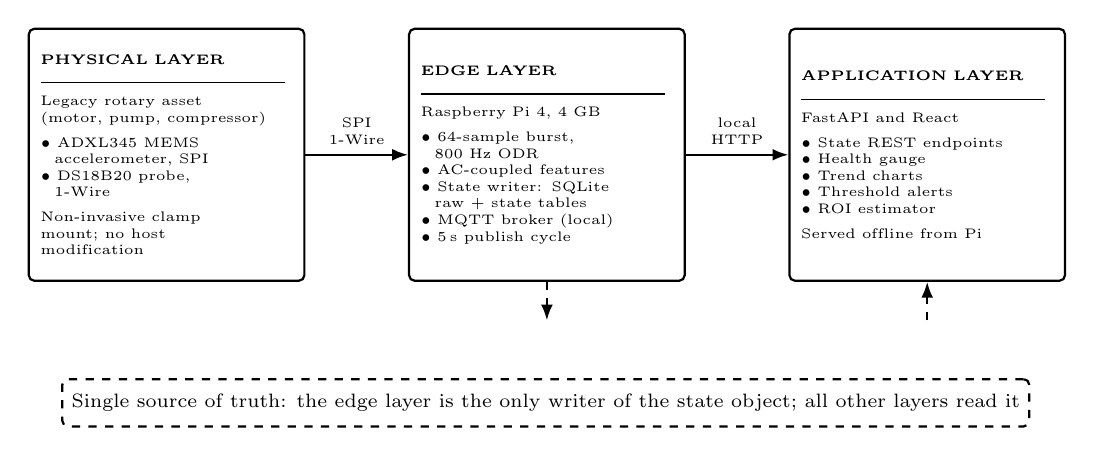
\begin{tikzpicture}[
  font=\tiny,
  layer/.style={rectangle, draw, thick, rounded corners=2pt,
                minimum width=3.5cm, minimum height=3.2cm,
                text width=3.2cm, align=left, anchor=north west},
  arr/.style={-{Latex[length=2mm]}, thick}
]

\node[layer] (phys) at (0,0) {
  \textbf{PHYSICAL LAYER}\\[1pt]
  \rule{3.1cm}{0.4pt}\\[2pt]
  Legacy rotary asset\\
  (motor, pump, compressor)\\[3pt]
  $\bullet$ ADXL345 MEMS\\
  \hspace{5pt}accelerometer, SPI\\
  $\bullet$ DS18B20 probe,\\
  \hspace{5pt}1-Wire\\[3pt]
  Non-invasive clamp\\
  mount; no host\\
  modification
};

\node[layer] (edge) at (4.83,0) {
  \textbf{EDGE LAYER}\\[1pt]
  \rule{3.1cm}{0.4pt}\\[2pt]
  Raspberry Pi 4, 4~GB\\[3pt]
  $\bullet$ 64-sample burst,\\
  \hspace{5pt}800~Hz ODR\\
  $\bullet$ AC-coupled features\\
  $\bullet$ State writer: SQLite\\
  \hspace{5pt}raw + state tables\\
  $\bullet$ MQTT broker (local)\\
  $\bullet$ 5\,s publish cycle
};

\node[layer] (app) at (9.66,0) {
  \textbf{APPLICATION LAYER}\\[1pt]
  \rule{3.1cm}{0.4pt}\\[2pt]
  FastAPI and React\\[3pt]
  $\bullet$ State REST endpoints\\
  $\bullet$ Health gauge\\
  $\bullet$ Trend charts\\
  $\bullet$ Threshold alerts\\
  $\bullet$ ROI estimator\\[3pt]
  Served offline from Pi
};

\draw[arr] (phys.east) -- node[above, align=center, font=\tiny]{SPI\\1-Wire} (edge.west);
\draw[arr] (edge.east) -- node[above, align=center, font=\tiny]{local\\HTTP} (app.west);

\node[draw, dashed, thick, rounded corners=2pt, anchor=north,
      minimum width=9.2cm, minimum height=0.6cm, align=center,
      font=\scriptsize] (sot) at (6.58,-4.45)
      {Single source of truth: the edge layer is the only writer of the state object; all other layers read it};

\draw[arr, dashed] (edge.south) -- ($(edge.south)+(0,-0.49)$);
\draw[arr, dashed] ($(app.south)+(0,-0.49)$) -- (app.south);

\end{tikzpicture}
\caption{Digital Cousin architecture as implemented in Phase~1. Every
element shown executes on the single edge node or on the sensors attached to
it, with no network egress on any path.}
\label{fig:arch}
\end{figure*}

\section{System Architecture}
\label{sec:arch}

Fig.~\ref{fig:arch} shows the four layers. We describe each in turn,
emphasising the choices the MSME constraint forced.

\subsection{Physical Layer and Retrofit}

Vibration is sensed with an ADXL345 three-axis MEMS accelerometer on a
GY-291 type breakout over SPI at 3.3~V; temperature with a waterproof
DS18B20 on a 1-Wire bus. The probe shell contains no pull-up, so the data
line needs one externally: a 4.7~k$\Omega$ resistor is the permanent
solution, while the host's internal GPIO pull-up also enumerates the device
but is lost on reboot, making it adequate for bench bring-up only. Both
sensors mount non-invasively on the bearing housing and motor casing, so no
hole is drilled and no alignment is disturbed. Rigid mounting matters more
than sensor grade, because a compliant mount low-pass-filters the very
transients the system looks for.

Two assembly details earn a place in the protocol because they cost us
bring-up time. The breakout's header pins must be soldered rather than
press-fitted: a header resting in its holes makes and breaks every
connection, power included, presenting as an intermittent rather than a dead
fault. The device-identity read localises that fault class, because such a
module returns an all-zero identity while the rails measure correct.

The register path follows the datasheet: a 3.9~mg/LSB full-resolution scale
factor and an explicit \texttt{POWER\_CTL}, \texttt{DATA\_FORMAT} and
\texttt{BW\_RATE} initialisation sequence, with the identity read as the
installation smoke test. The acquisition rate warrants a precise statement,
since it is easily misread as a shortfall. The ADXL345 supports output data
rates to 3,200~Hz in SPI mode; this system \emph{configures} 800~Hz by
writing \texttt{BW\_RATE} and takes a 64-sample burst paced at that rate.
That is a deliberate scoping decision, not a rate the implementation failed
to reach. Continuous high-rate streaming is deferred because sustaining it
from a managed-runtime service is a real-time scheduling problem of
buffering and jitter, better tuned against the pilot machine than claimed in
advance. Section~\ref{sec:limits} states the consequence: signatures above
roughly 5~kHz, which envelope analysis \cite{b9} targets, need 10~kHz and
above and are out of scope.

A battery-backed DS3231 real-time clock is specified and budgeted in
Table~\ref{tab:bom}, though not yet fitted on the bench unit. The Raspberry
Pi has no on-board clock and would otherwise restore a stale time at boot
and depend on a network time source to correct it, a dependency incompatible
with P2 that undermines the state object directly, since every record is
keyed by \texttt{timestamp}. Fitting it is a prerequisite for unattended
deployment.

\subsection{Edge Layer}

A Raspberry Pi 4 with 4~GB of RAM hosts acquisition, feature extraction,
persistence and messaging. Four features are computed per burst, each over
the AC-coupled signal: RMS, kurtosis, crest factor and peak-to-peak. AC
coupling is not incidental: the window mean is dominated by the roughly 1~g
gravity component at any mount orientation, and subtracting it first is the
difference between measuring vibration and measuring mount angle. Kurtosis
follows Pearson's definition, so baseline sits near 3.0.

A single publish cycle, five seconds by default and configurable, reads both
sensors in one call, so vibration features and temperature are persisted
together at 0.2~Hz. One cycle writing one object keeps the state object
atomic and its timestamp meaningful. Both the period and the burst are
scheduled against running deadlines rather than slept for a fixed interval,
because acquisition is not instantaneous: the DS18B20 alone needs roughly
750~ms for a 12-bit conversion. Under the naive formulation that time is
additive, and the deployed system measured 6.00~s per cycle and 751~Hz per
burst against configured values of 5~s and 800~Hz. Deadline scheduling
removes the drift: 5.000~s (0.2000~Hz) and 799.4~Hz measured. Persistence
uses SQLite in two deliberately separate tables: \texttt{raw\_readings}
records what the sensor reported, \texttt{state\_history} the full state
object including the fields that are null in this phase. Keeping them apart
means the raw record never acquires placeholder values for quantities that
did not exist when it was written. Two MQTT topics mirror the split on a
local broker; the publish path is implemented against both, while the bench
results reported here came through the SQLite store with no broker
resident.

\subsection{Application Layer}

A FastAPI service and a React single-page application compose the
user-facing system, served from the Pi over the local network by nginx
rather than a development server. Two endpoints expose the twin: current
state and bounded history. The dashboard renders a health gauge, vibration
and temperature trends, an active-alert panel and a filterable history log,
using inline SVG rather than a charting dependency to keep the offline
bundle small. Alerting is deterministic in Phase~1, applying configurable
upper and lower thresholds and surfacing breaches in the alert panel; a
GPIO-driven piezo buzzer is specified and budgeted but is not part of the
software reported here. The model's alert level joins the threshold path in
Phase~2, surfaced alongside rather than replacing it. A client-side ROI
estimator converts operator-supplied downtime cost and annual unplanned
hours into a projected saving.

The memory budget is what makes the phase boundary credible. Phase~1
occupies roughly 750~MB resident against 4~GB installed: 400~MB for Raspberry
Pi OS Lite, 150~MB for acquisition and the broker, 100~MB for SQLite and
100~MB for the API and dashboard.

\subsection{Bill of Materials}

Table~\ref{tab:bom} gives the per-deployment bill of materials for the
shop-floor configuration, approximately INR 20,000 including contingency.
The figure is one-time: no licence, no subscription, no metered egress, so
five-year ownership is the purchase price plus electricity, against a cloud
alternative whose charges are recurring and quote-based. It is also the
\emph{full} configuration. The sensing and compute core alone is roughly
INR 7,600 and a headless variant approximately INR 12,200. We quote the
larger figure throughout because the touchscreen is what makes P3 real on a
floor where the operator has no laptop.

\begin{table}[t]
\caption{Per-Deployment Bill of Materials, Shop-Floor Configuration}
\label{tab:bom}
\centering
\footnotesize
\setlength{\tabcolsep}{3pt}
\begin{tabular}{|p{2.9cm}|p{2.6cm}|r|}
\hline
\textbf{Component} & \textbf{Part or specification} & \textbf{INR} \\
\hline
Vibration sensor & ADXL345 breakout, SPI & 250 \\
Temperature sensor & DS18B20 waterproof & 200 \\
Pull-up and passives & 4.7~k$\Omega$, decoupling & 50 \\
Edge compute & Raspberry Pi 4, 4~GB & 6,500 \\
Real-time clock & DS3231, battery-backed & 200 \\
Power supply & 5~V, 3~A USB-C & 800 \\
Power buffering & UPS HAT, 2 cells & 1,600 \\
Storage & 32~GB Class-10 card & 400 \\
Operator HMI & 7-inch touchscreen & 4,800 \\
Enclosure & IP54 box, DIN rail & 1,200 \\
Sensor mounting & Magnetic fixture & 600 \\
Interconnect & 3~m shielded cable & 500 \\
Audible alert & Piezo buzzer, driver & 150 \\
Thermal & Heatsink case, fan & 600 \\
Consumables & Jumpers, fasteners & 350 \\
\hline
\textbf{Subtotal} & & \textbf{18,200} \\
Contingency and spares & 10\% & 1,820 \\
\hline
\textbf{Total per deployment} & & \textbf{20,020} \\
\hline
\multicolumn{3}{p{0.95\columnwidth}}{\scriptsize Indicative Indian retail
prices at the procurement window, not quotations. Software cost is zero;
the headless configuration is approximately INR 12,200 and the sensing and
compute core INR 7,600.} \\
\end{tabular}
\end{table}

\section{Evaluation Methodology}
\label{sec:eval}

Table~\ref{tab:eval} states every Phase~1 metric, its pre-registered target
and its current status. We set targets out in full because a stated target
later missed is informative, while one chosen after the fact is not. Rows
depending on the pilot machine remain TBD; architectural and cost
properties, determined by design rather than measurement, are reported as
established.

\begin{table}[t]
\caption{Phase 1 Metrics, Pre-Registered Targets and Status}
\label{tab:eval}
\centering
\footnotesize
\setlength{\tabcolsep}{3pt}
\begin{tabular}{|p{3.4cm}|p{1.9cm}|p{1.4cm}|}
\hline
\textbf{Metric} & \textbf{Target} & \textbf{Status} \\
\hline
\multicolumn{3}{|l|}{\emph{Retrofit and hardware}} \\
\hline
Device identity read & pass & \textbf{pass} \\

Retrofit with no host modification & pass or fail & TBD \\
Vibration RMS vs.\ reference instrument & within $\pm 10\%$ & TBD \\
Temperature vs.\ traceable thermometer & within $\pm 1^{\circ}$C & TBD \\
Baseline recording duration & 30 min & TBD \\
Second-installer reproduction & pass or fail & TBD \\
\hline
\multicolumn{3}{|l|}{\emph{Acquisition and runtime}} \\
\hline
Configured burst ODR & 800 Hz & \textbf{800 Hz} \\
Publish period, both channels & 5 s & \textbf{5.000 s} \\
Effective publish rate & 0.2 Hz & \textbf{0.2000 Hz} \\
Effective burst rate & 800 Hz & \textbf{799.4 Hz} \\
Steady-state resident memory & $\leq 1$ GB & \textbf{282 MB} \\
Dashboard load over local network & $\leq 3$ s & \textbf{0.06 s} \\
Continuous uptime, soak test & not set & TBD \\
\hline
\multicolumn{3}{|l|}{\emph{System and cost}} \\
\hline
Full function with no network egress & pass or fail & TBD \\
Total per-deployment cost & $\leq$ INR 20,000 & INR 20,020 \\
ROI projection vs.\ manual calculation & within $\pm 5\%$ & TBD \\
\hline
\multicolumn{3}{p{0.95\columnwidth}}{\scriptsize Measured on the deployment
hardware (Raspberry Pi 4 Rev 1.5), both channels live. Memory is
whole-system resident, the services accounting for 150~MB; the dashboard is
a 169~KB build over the local network. TBD rows need a reference instrument
or an installed asset.} \\
\end{tabular}
\end{table}

\section{Results}
\label{sec:results}

\subsection{Settled Results and Bring-Up Findings}

Phase~1 is verified end to end on the deployment hardware with both sensors
attached. The DS18B20 returns CRC-valid readings matching the temperature
the API serves, and the ADXL345 responds to physical excitation: over 15
consecutive records the features take 15 distinct values, and deliberate
taps register as impulsive transients, kurtosis rising from a 2.4--3.8
baseline to 8.38 and peak-to-peak from 0.06~g to 0.14~g while RMS barely
moves. That is the signature those two statistics exist to detect. All five
model-derived fields are null in every record, which is the state-object
contract of Section~\ref{sec:state} holding in practice.

The device-identity read passes on the deployment hardware. It \emph{failed}
on the first wiring attempt, caused by the unsoldered header of
Section~\ref{sec:arch}, and passed once soldered. We report the failure
rather than the eventual pass, because the check earning its place in the
protocol is the finding: without an explicit identity gate, a well-formed
all-zero identity propagates as plausible data rather than as an error.

\subsection{Comparison with Existing Approaches}

Comparison is organised against three reference classes, since no prior
system occupies this design point. Against \emph{commercial twin platforms}
the advantage is structural: no industrial protocol is required on the
asset, which is what makes a non-instrumented lathe addressable at all;
there is no licence or consumption charge against a sector with the credit
constraint documented in \cite{b37}; and the system functions with the
network disconnected. Against \emph{edge and TinyML monitors}
\cite{b16,b17,b20} it concedes resource efficiency, since a Raspberry Pi is
a far larger budget than an ESP32, and spends it on an operator-facing
application layer those systems do not attempt. Against \emph{brownfield SME
twin frameworks} \cite{b5} it carries the conceptual scoping through to a
running system and a published bill of materials.

\section{Discussion}

Two aspects of the design generalise beyond this deployment.

\textbf{Narrow scope is an enabling constraint.} Accepting a single asset
does not merely reduce cost; the ontology-maintenance burden it removes is
precisely what makes knowledge-graph-driven twins impractical for a firm
with no IT staff. The state model collapses to one object with a single
writer, which is what will make the Phase~2 retrieval context small enough
to fit entirely in a sub-2B-parameter model's prompt without embedding
infrastructure. The chain from P1 to P3 is causal, not coincidental.

\textbf{Cost structure, not unit cost, is what excludes MSMEs.} A firm that
can find INR 20,000 once may still be unable to commit to a recurring
per-asset charge \cite{b33,b34}; designing for zero recurring cost is a
different objective from designing for low cost, and it is the one the
edge-first property serves.

\section{Limitations}
\label{sec:limits}

These are binding constraints on how the results should be read, not caveats
to be discounted. \textbf{Sampling bandwidth:} the configured rate is 800~Hz
in 64-sample bursts against a 3,200~Hz part ceiling, so signatures above
roughly 5~kHz and the envelope analysis targeting them \cite{b9} are
unavailable; the system addresses low- and mid-frequency degradation and
should not be represented as performing spectral bearing diagnosis.
\textbf{Bring-up is complete on the bench, not on a pilot machine:} both
channels are verified end to end on the deployment hardware and the
accelerometer passes its identity check, but validation against a reference
instrument on an installed asset remains, and it gates the rows marked TBD
in Table~\ref{tab:eval}.
\textbf{Single asset, single site:} the evaluation is a controlled pilot,
so adoption friction, installer variability and the accuracy of the cost
figures at scale remain open.
\textbf{Historical window bound:} the history endpoint is capped at 1,000
rows rather than a true time range, which at the default five-second
interval corresponds to under 1.4~hours; extending it requires pagination
and time-range support. Finally, anomaly scoring, health indexing,
prognostics and the operator-facing interface are Phase~2, and no claim here
rests on them.

\section{Conclusion and Future Work}
\label{sec:conc}

We have presented Digital Cousin, a digital twin for a single legacy machine
running entirely on a Raspberry Pi 4, and reported Phase~1: the non-invasive
retrofit, the deterministic edge acquisition path and the digital shadow on
which the analytics and operator interface are built. Its three properties are
single-asset scope, edge-first execution and natural-language accessibility.
Together they form a coherent design point rather than a reduced enterprise
twin, reachable at approximately INR 20,000 of one-time hardware with no
licence and no cloud dependency. The finding that an unsoldered
header presents as a well-formed all-zero device identity has been folded
back into the retrofit protocol.

Phase~2 populates the five reserved fields with on-device analytics trained
on CWRU \cite{b7} and IMS \cite{b8} and adds the operator-facing language
interface. Two further directions follow from Phase~1 itself. A non-invasive
current clamp would add an electrically grounded fault channel covering
phase imbalance and overload, complementary to vibration and cheap to
retrofit. And a multi-site field study with MSME partners would turn a pilot
into an adoption pathway, the step the adoption literature identifies as
missing \cite{b33,b34,b35}.

\section*{Acknowledgment}

The authors thank Dayananda Sagar University for institutional support. No
external funding was received.

\begin{thebibliography}{00}

\bibitem{b1}
F. Tao, H. Zhang, A. Liu, and A. Y. C. Nee, ``Digital twin in industry:
State-of-the-art,'' \textit{IEEE Trans. Ind. Informat.}, vol. 15, no. 4,
pp. 2405--2415, Apr. 2019.

\bibitem{b2}
J. Lee, B. Bagheri, and H.-A. Kao, ``A cyber-physical systems architecture
for Industry 4.0-based manufacturing systems,'' \textit{Manuf. Lett.},
vol. 3, pp. 18--23, Jan. 2015.

\bibitem{b3}
R. van Dinter, B. Tekinerdogan, and C. Catal, ``Reference architecture for
digital twin-based predictive maintenance systems,'' \textit{Comput. Ind.
Eng.}, vol. 177, art. 109099, Mar. 2023.

\bibitem{b4}
J. Leng, Q. Liu, S. Ye, J. Jing, Y. Wang, C. Zhang, D. Zhang, and X. Chen,
``Digital twin-driven rapid reconfiguration of the automated manufacturing
system via an open architecture model,'' \textit{Robot. Comput.-Integr.
Manuf.}, vol. 63, art. 101895, 2020.

\bibitem{b5}
S. Krommes and F. Tomaschko, ``Conceptual framework of a digital twin
fostering sustainable manufacturing in a brownfield approach of small volume
production for SMEs,'' in \textit{Manufacturing Driving Circular Economy
(GCSM 2022)}, Lecture Notes in Mechanical Engineering. Cham, Switzerland:
Springer, 2023, pp. 519--527.

\bibitem{b6}
A. Gautam, M. R. Aryal, S. Deshpande, S. Padalkar, M. Nikolaenko, M. Tang,
and S. Anand, ``IIoT-enabled digital twin for legacy and smart factory
machines with LLM integration,'' \textit{J. Manuf. Syst.}, vol. 80,
pp. 511--523, 2025.

\bibitem{b7}
W. A. Smith and R. B. Randall, ``Rolling element bearing diagnostics using
the Case Western Reserve University data: A benchmark study,'' \textit{Mech.
Syst. Signal Process.}, vols. 64--65, pp. 100--131, 2015.

\bibitem{b8}
H. Qiu, J. Lee, J. Lin, and G. Yu, ``Wavelet filter-based weak signature
detection method and its application on rolling element bearing
prognostics,'' \textit{J. Sound Vib.}, vol. 289, no. 4--5, pp. 1066--1090,
2006.

\bibitem{b9}
R. B. Randall and J. Antoni, ``Rolling element bearing diagnostics: A
tutorial,'' \textit{Mech. Syst. Signal Process.}, vol. 25, no. 2,
pp. 485--520, 2011.

\bibitem{b10}
R. Zhao, R. Yan, Z. Chen, K. Mao, P. Wang, and R. X. Gao, ``Deep learning
and its applications to machine health monitoring,'' \textit{Mech. Syst.
Signal Process.}, vol. 115, pp. 213--237, 2019.

\bibitem{b11}
H.-X. Hu, Y. Feng, Q. Hu, and Y. Zhang, ``A masked one-dimensional
convolutional autoencoder for bearing fault diagnosis based on digital twin
enabled industrial internet of things,'' \textit{IEEE J. Sel. Areas
Commun.}, vol. 41, no. 10, pp. 3242--3253, 2023.

\bibitem{b12}
F. T. Liu, K. M. Ting, and Z.-H. Zhou, ``Isolation forest,'' in \textit{Proc.
8th IEEE Int. Conf. Data Mining (ICDM)}, Pisa, Italy, 2008, pp. 413--422.

\bibitem{b13}
F. Yuan, C. Zhang, and X. Liu, ``Bearing fault diagnosis based on
auto-encoder combined with CNN,'' in \textit{Fuzzy Systems and Data Mining
IX}, Frontiers in Artificial Intelligence and Applications, vol. 354.
Amsterdam, The Netherlands: IOS Press, 2023, pp. 334--344.

\bibitem{b15}
E. Njor, M. A. Hasanpour, J. Madsen, and X. Fafoutis, ``A holistic review of
the TinyML stack for predictive maintenance,'' \textit{IEEE Access},
vol. 12, pp. 184861--184882, 2024.

\bibitem{b16}
M. Antonini, M. Pincheira, M. Vecchio, and F. Antonelli, ``An adaptable and
unsupervised TinyML anomaly detection system for extreme industrial
environments,'' \textit{Sensors}, vol. 23, no. 4, art. 2344, 2023.

\bibitem{b17}
Z. Chen, Y. Gao, and J. Liang, ``LOPdM: A low-power on-device predictive
maintenance system based on self-powered sensing and TinyML,'' \textit{IEEE
Trans. Instrum. Meas.}, vol. 72, pp. 1--13, 2023.

\bibitem{b20}
J. Pournazari, M. El-Dalahmeh, A. Al-Dubai, X. Liu, D.-H. Park, J. Marco,
T. Q. Dinh, J.-H. Ahn, and M. Faraji Niri, ``LiRUL: A physics-constrained
and lightweight learning framework for edge-based RUL prediction,''
\textit{Results Eng.}, 2026.

\bibitem{b23}
S. V. Kandala, P. Medaranga, and A. Varshney, ``TinyLLM: A framework for
training and deploying language models at the edge computers,''
arXiv:2412.15304, 2024.

\bibitem{b24}
T. An, Y. Zhou, H. Zou, and J. Yang, ``IoT-LLM: A framework for enhancing
large language model reasoning from real-world sensor data,''
\textit{Patterns}, 2025.

\bibitem{b25}
J. Jeon, Y. Sim, H. Lee, C. Han, D. Yun, and E. Kim, ``ChatCNC:
Conversational machine monitoring via large language model and real-time
data retrieval augmented generation,'' \textit{J. Manuf. Syst.}, vol. 79,
pp. 504--514, 2025.

\bibitem{b26}
H. Peng, J. Liu, J. Du, J. Gao, and W. Wang, ``BearLLM: A prior
knowledge-enhanced bearing health management framework with unified
vibration signal representation,'' in \textit{Proc. AAAI Conf. Artif.
Intell.}, vol. 39, no. 19, 2025, pp. 19866--19874.

\bibitem{b27}
Y. Xia, D. Dittler, N. Jazdi, H. Chen, and M. Weyrich, ``LLM experiments
with simulation: Large language model multi-agent system for process
simulation parametrization in digital twins,'' in \textit{Proc. 29th IEEE
Int. Conf. Emerg. Technol. Factory Autom. (ETFA)}, 2024; arXiv:2405.18092.

\bibitem{b33}
A. Raj, G. Dwivedi, A. Sharma, A. B. L. de Sousa Jabbour, and S. Rajak,
``Barriers to the adoption of industry 4.0 technologies in the manufacturing
sector: An inter-country comparative perspective,'' \textit{Int. J. Prod.
Econ.}, vol. 224, art. 107546, 2020.

\bibitem{b34}
K. L. Gold, ``Effects of Industry 4.0 on small and medium-scale enterprises:
An analytical and bibliometric review,'' \textit{SAGE Open}, vol. 15, no. 2,
2025.

\bibitem{b35}
S. O. Ooko and S. M. Karume, ``Application of tiny machine learning in
predicative maintenance in industries,'' \textit{J. Comput. Theories Appl.},
vol. 2, no. 1, pp. 131--150, 2024.

\bibitem{b36}
Ministry of Micro, Small and Medium Enterprises, Government of India,
\textit{Annual Report 2023--24}. New Delhi, India: Government of India,
2024.

\bibitem{b37}
International Finance Corporation and Intellecap, \textit{Financing India's
MSMEs: Estimation of Debt Requirement of MSMEs in India}. Washington, DC,
USA: World Bank Group, 2018.

\end{thebibliography}

\end{document}
